\documentclass[12pt,a4paper]{article}

% This report follows the exact preamble and cover formatting of reference.tex.
\usepackage[utf8]{inputenc}
\usepackage[T1]{fontenc}
\usepackage{geometry}
\usepackage{xcolor}
\usepackage{listings}
\usepackage{amsmath,amssymb}
\usepackage{graphicx}
\usepackage{booktabs}
\usepackage{array}
\usepackage{enumitem}
\usepackage{hyperref}
\usepackage{float}
\usepackage{eso-pic}

\geometry{left=2.5cm, right=2.5cm, top=2.5cm, bottom=2.5cm}

\lstdefinestyle{plain}{
  basicstyle=\ttfamily\small,
  numberstyle=\tiny,
  numbers=left, numbersep=6pt,
  frame=none,
  breaklines=true, showstringspaces=false,
  tabsize=2, captionpos=b,
  xleftmargin=18pt,
  aboveskip=10pt, belowskip=6pt
}

\lstdefinestyle{code}{
  basicstyle=\ttfamily\footnotesize,
  numberstyle=\tiny\color{gray},
  numbers=left, numbersep=6pt,
  frame=single,
  breaklines=true, showstringspaces=false,
  tabsize=4, captionpos=b,
  xleftmargin=18pt,
  aboveskip=10pt, belowskip=10pt,
  language=Python,
  keywordstyle=\color{blue!60!black}\bfseries,
  commentstyle=\color{green!40!black}\itshape,
  stringstyle=\color{orange!70!black},
}

\setcounter{secnumdepth}{0}
\pagestyle{plain}
\hypersetup{colorlinks=true, linkcolor=black, urlcolor=black}

\begin{document}

% Cover page based on reference.tex.
\thispagestyle{empty}
\AddToShipoutPictureBG{%
  \AtPageLowerLeft{%
    \hspace{1.2cm}\raisebox{1.2cm}{%
      \color{black}\framebox[\dimexpr\paperwidth-2.4cm\relax]{%
        \rule{0pt}{\dimexpr\paperheight-2.4cm\relax}}%
    }%
  }%
}

\begin{center}

\vspace*{1.4cm}

\includegraphics[width=0.22\textwidth]{outputs/emblem.png}\\[0.6cm]

{\Large TRIBHUVAN UNIVERSITY}\\[0.35cm]
{\large INSTITUTE OF ENGINEERING}\\[0.15cm]
{\large PULCHOWK CAMPUS}\\[1.4cm]

{\bfseries\large A LAB REPORT\\
ON\\[0.2cm]
Artificial Neural Networks: McCulloch-Pitts, Adaline and Backpropagation}

\vspace{2.2cm}
{\rule{0.3pt}{2.3cm}}\hspace{1.4cm}{\rule{0.3pt}{2.3cm}}\hspace{1.4cm}{\rule{0.3pt}{2.3cm}}

\vspace{2.6cm}
\end{center}

\noindent
\begin{minipage}[t]{0.47\textwidth}
\vspace{0pt}
\underline{\textbf{SUBMITTED BY:}}\\[0.4cm]
Name: Aditya Kumar Shah\\[0.2cm]
Roll No.: 080BCT011\\[0.2cm]
Lab No.: 07
\end{minipage}\hfill
\begin{minipage}[t]{0.47\textwidth}
\vspace{0pt}
\begin{flushright}
\underline{\textbf{SUBMITTED TO:}}\\[0.4cm]
Department of Electronics\\[0.2cm]
and Computer Engineering
\end{flushright}
\end{minipage}

\vfill
\newpage

\section*{1. Objectives}

\begin{enumerate}[leftmargin=1.6em]
  \item To design a McCulloch-Pitts neuron trained with Adaline (delta rule) learning that behaves as a 2-input AND gate, and to study the effect of its learning parameters.
  \item To extend the same Adaline learning procedure to OR, NAND and NOR gates and to draw the resulting neural nets.
  \item To repeat the Adaline experiments using the bipolar ($-1/1$) encoding and compare it with the unipolar ($0/1$) encoding.
  \item To implement a McCulloch-Pitts network for the XOR function, which is not linearly separable, and to state the formulas used.
  \item To implement and train a multilayer perceptron (MLP) for XOR using the backpropagation algorithm.
\end{enumerate}

\section*{2. Theoretical Background}

An Adaline (Adaptive Linear Neuron) unit computes a net input $y\_in = b + \sum_i x_i w_i$ and is trained with the delta rule (least mean squares / Widrow-Hoff rule):
\[
  b(\text{new}) = b(\text{old}) + \alpha(t - y\_in), \qquad
  w_i(\text{new}) = w_i(\text{old}) + \alpha(t - y\_in)x_i .
\]
Training stops when the largest weight/bias change in an epoch falls below a tolerance, or a maximum number of epochs is reached. After training, the class is decided by a threshold applied to $y\_in$: for the unipolar case the unit fires ($y=1$) if $y\_in > 0.5$, and for the bipolar case it fires ($y=1$) if $y\_in \geq 0$, otherwise $y=-1$.

A single Adaline/perceptron unit can only realize linearly separable functions. AND, OR, NAND and NOR are linearly separable and can therefore be learned directly. XOR is not linearly separable, so it requires either a fixed-weight McCulloch-Pitts network built from simpler gates, or a multilayer network with a hidden layer trained by backpropagation, as also noted in the lab sheet.

For the backpropagation algorithm, with sigmoid activation $f(x) = 1/(1+e^{-x})$ (so $f'(x) = f(x)(1-f(x))$), each pattern is used to update the weights as follows:
\[
  \delta_k = (t_k - y_k) f'(y\_in_k), \qquad
  \delta\_in_j = \sum_k \delta_k w_{jk}, \qquad
  \delta_j = \delta\_in_j\, f'(z\_in_j),
\]
\[
  \Delta w_{jk} = \alpha \delta_k z_j, \qquad
  \Delta w_{ij} = \alpha \delta_j x_i, \qquad
  w(\text{new}) = w(\text{old}) + \Delta w .
\]

\section*{3. Assignment 1 --- AND Gate using Adaline (Unipolar)}

A single Adaline unit with two inputs and a bias was trained on the unipolar AND truth table using the delta-rule update above, with learning rate $\alpha = 0.1$, small random initial weights, and a stopping tolerance of $10^{-3}$ on the largest weight change (run for a maximum of 500 epochs). The unit converged to the correct classification for all four patterns.

\begin{center}
\begin{tabular}{@{}lrrrr@{}}
\toprule
\textbf{Gate} & $w_1$ & $w_2$ & $b$ & \textbf{Epochs to correct classification} \\
\midrule
AND (unipolar) & 0.556 & 0.528 & $-0.278$ & 2 \\
\bottomrule
\end{tabular}
\end{center}

\begin{figure}[H]
\centering
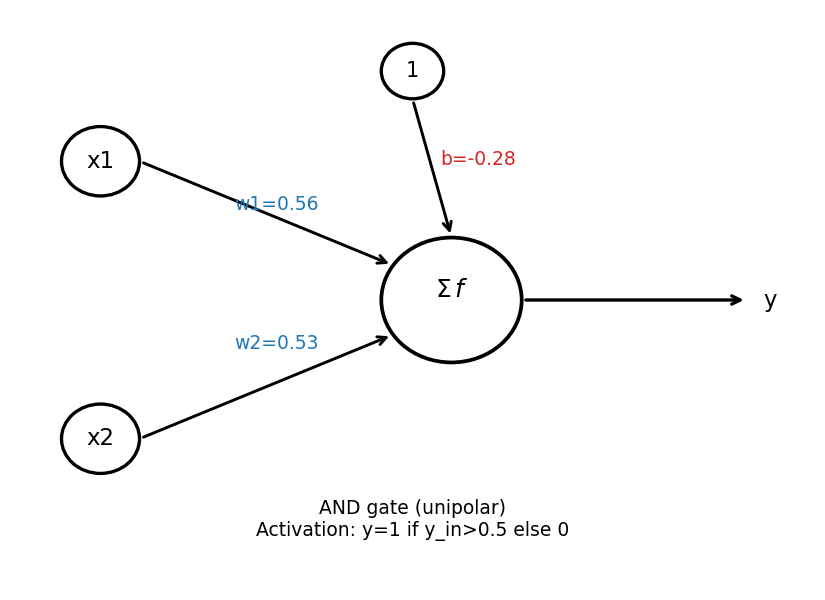
\includegraphics[width=0.55\textwidth]{outputs/neuron_and_unipolar.png}
\caption{McCulloch-Pitts/Adaline neuron trained as an AND gate (unipolar), with final weights and bias.}
\end{figure}

\subsection*{3.1 Parameter Variation}

To study the effect of the learning rate and the initial weight scale on convergence speed, the AND gate was retrained for $\alpha \in \{0.01, 0.05, 0.1, 0.3, 0.5, 0.9\}$ and for initial-weight scales in $\{0.1, 0.5, 1.0, 2.0\}$, each averaged over five random seeds. The number of epochs needed before the network first classifies all four patterns correctly was recorded.

\begin{figure}[H]
\centering
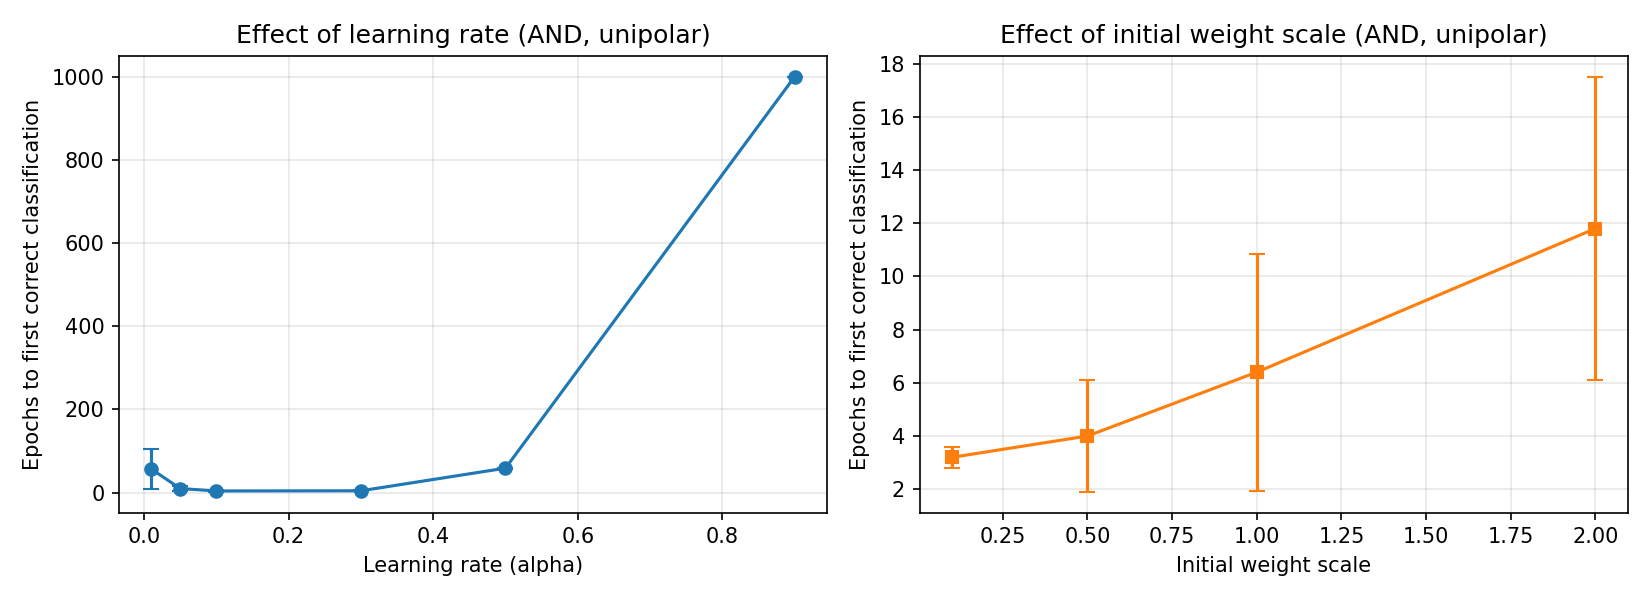
\includegraphics[width=0.92\textwidth]{outputs/param_study.png}
\caption{Effect of learning rate and initial weight scale on convergence speed for the AND gate (unipolar Adaline).}
\end{figure}

The results show a clear U-shaped dependence on the learning rate: a very small rate ($\alpha=0.01$) is slow because the weight updates are tiny (about 57 epochs on average); a moderate rate ($\alpha \approx 0.1$--$0.3$) converges fastest (about 4 epochs); and a large rate ($\alpha=0.9$) makes the weight updates overshoot so much that the SSE oscillates and the unit never settles into the correct classification within 1000 epochs. Larger initial weight magnitudes also slow convergence slightly, since the starting point is farther from the region where all four patterns are already classified correctly.

\section*{4. Assignment 2 --- OR, NAND and NOR Gates using Adaline}

The same Adaline trainer (delta rule, $\alpha=0.1$, unipolar encoding) was reused for OR, NAND and NOR by only changing the target vector.

\begin{center}
\begin{tabular}{@{}lrrrr@{}}
\toprule
\textbf{Gate} & $w_1$ & $w_2$ & $b$ & \textbf{Epochs to correct classification} \\
\midrule
OR   &  0.444 &  0.472 &  0.278 & 4  \\
NAND & $-0.556$ & $-0.528$ &  1.278 & 12 \\
NOR  & $-0.444$ & $-0.472$ &  0.722 & 22 \\
\bottomrule
\end{tabular}
\end{center}

\begin{figure}[H]
\centering
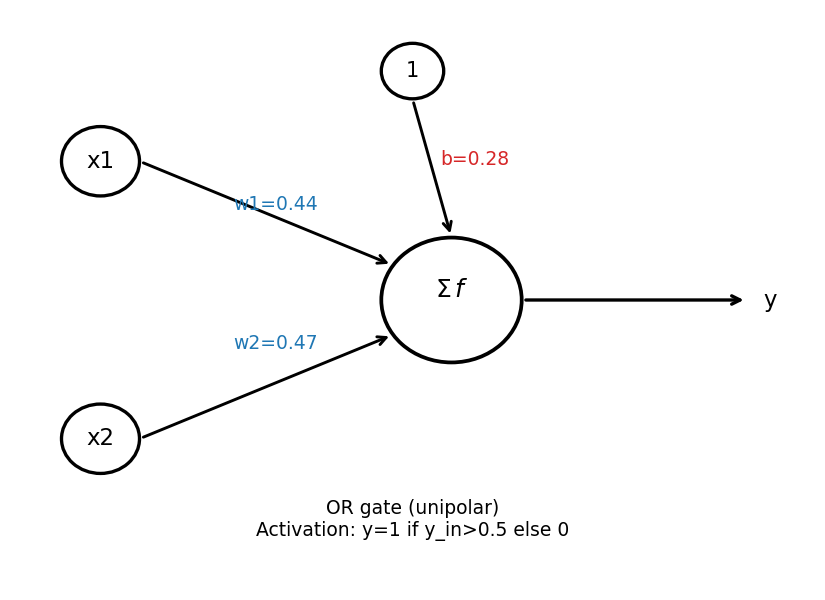
\includegraphics[width=0.48\textwidth]{outputs/neuron_or_unipolar.png}
\hspace{0.02\textwidth}
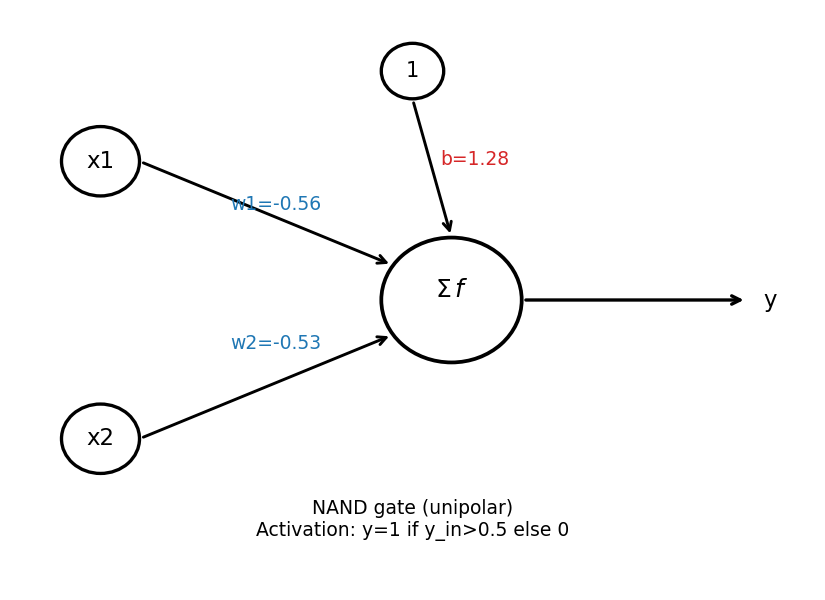
\includegraphics[width=0.48\textwidth]{outputs/neuron_nand_unipolar.png}\\[0.3cm]
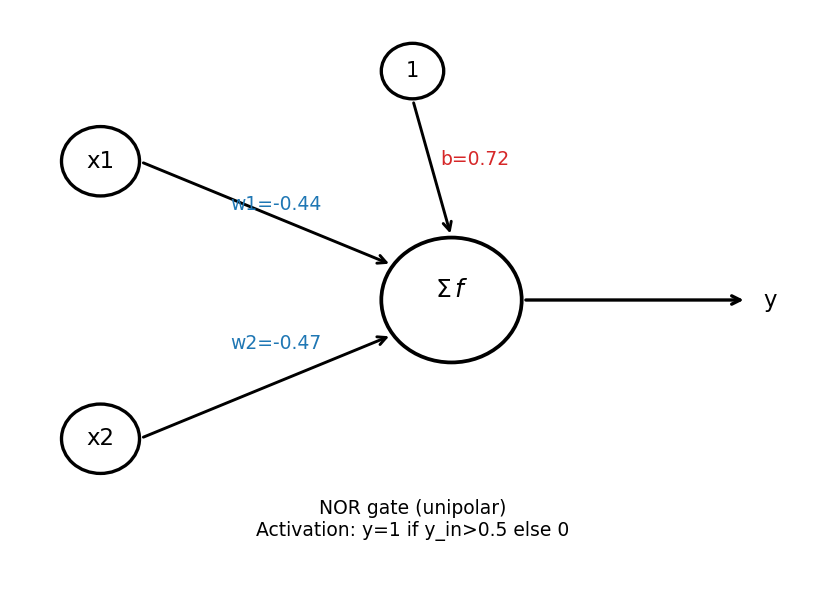
\includegraphics[width=0.48\textwidth]{outputs/neuron_nor_unipolar.png}
\caption{Adaline neurons trained as OR, NAND and NOR gates (unipolar), with final weights and bias.}
\end{figure}

\begin{figure}[H]
\centering
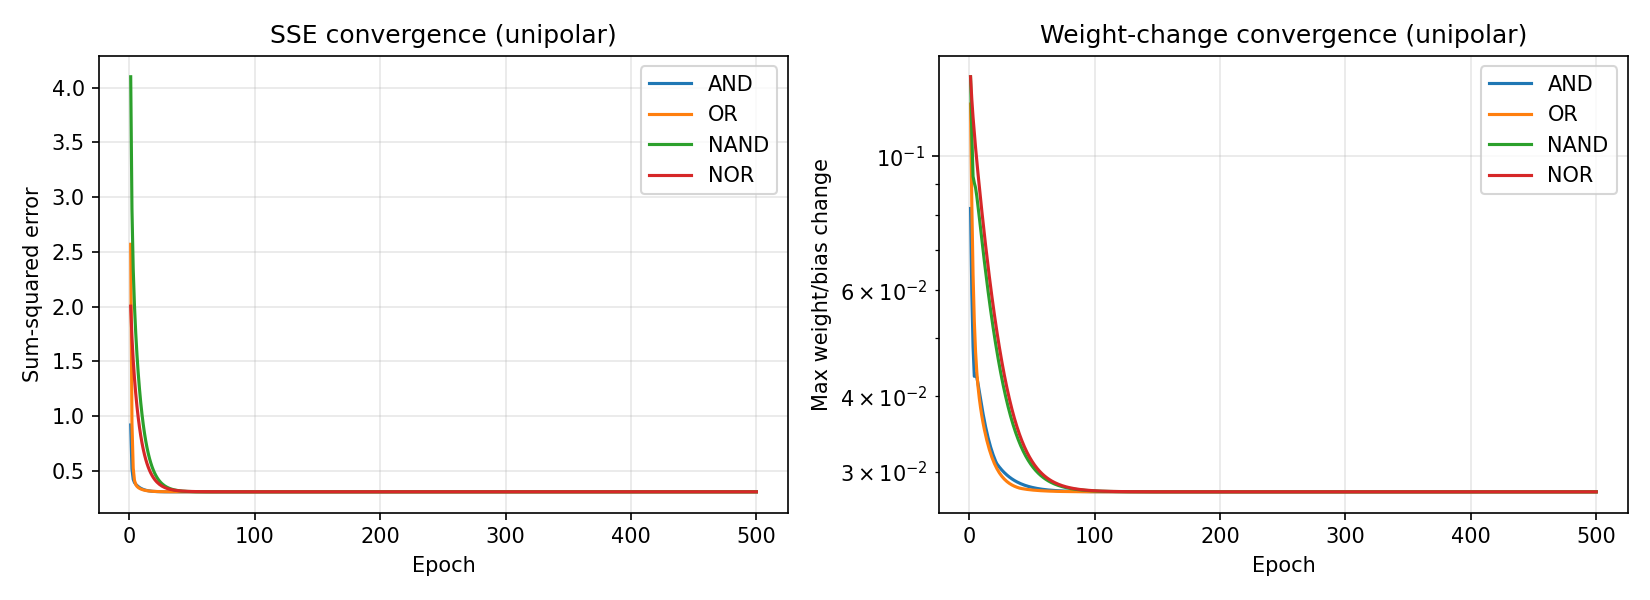
\includegraphics[width=0.92\textwidth]{outputs/unipolar_convergence.png}
\caption{Sum-squared error and weight-change convergence for AND, OR, NAND and NOR (unipolar Adaline, $\alpha=0.1$).}
\end{figure}

NAND and NOR take visibly more epochs to reach the correct classification than AND and OR (12 and 22 epochs versus 2 and 4). This happens because NAND/NOR require the bias to dominate the net input for three of the four patterns (i.e. the decision boundary sits close to a corner of the input square), so the delta rule needs more updates to push the bias far enough from its small random initial value.

\section*{5. Assignment 3 --- Bipolar Model}

The AND, OR, NAND and NOR experiments were repeated with the bipolar ($-1/1$) encoding for both inputs and targets, using the same learning rate and stopping rule.

\begin{center}
\begin{tabular}{@{}lrrrr@{}}
\toprule
\textbf{Gate} & $w_1$ & $w_2$ & $b$ & \textbf{Epochs to correct classification} \\
\midrule
AND  &  0.529 &  0.559 & $-0.5$ & 1 \\
OR   &  0.471 &  0.441 &  0.5 & 2 \\
NAND & $-0.529$ & $-0.559$ &  0.5 & 2 \\
NOR  & $-0.471$ & $-0.441$ & $-0.5$ & 3 \\
\bottomrule
\end{tabular}
\end{center}

\begin{figure}[H]
\centering
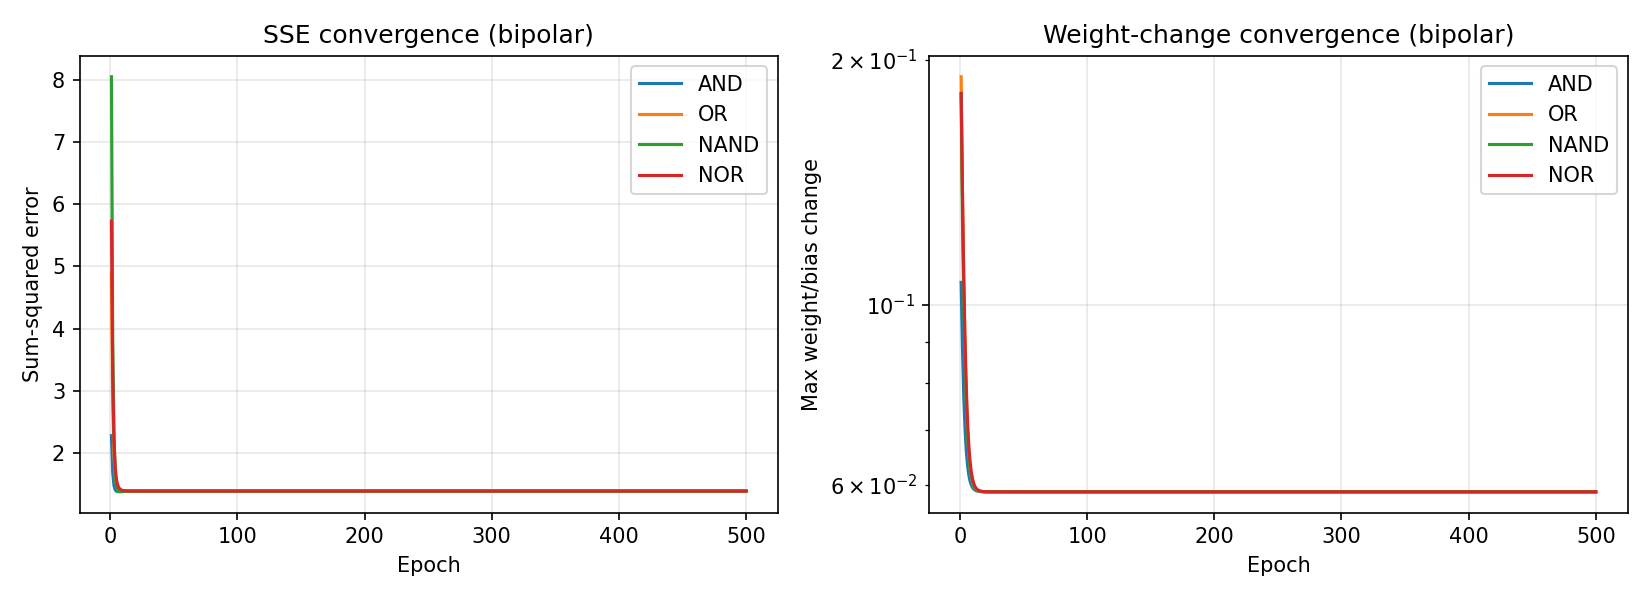
\includegraphics[width=0.92\textwidth]{outputs/bipolar_convergence.png}
\caption{Sum-squared error and weight-change convergence for AND, OR, NAND and NOR (bipolar Adaline, $\alpha=0.1$).}
\end{figure}

\begin{figure}[H]
\centering
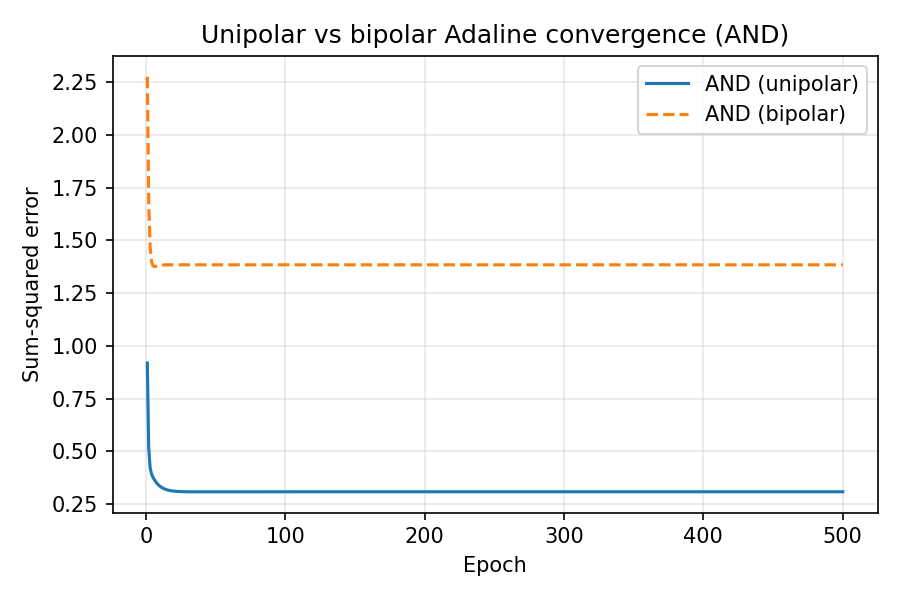
\includegraphics[width=0.7\textwidth]{outputs/unipolar_vs_bipolar_and.png}
\caption{Unipolar vs. bipolar convergence for the AND gate.}
\end{figure}

Every gate converges markedly faster with the bipolar encoding (1--3 epochs) than with the unipolar encoding (2--22 epochs). The reason is that unipolar inputs use $0$ to represent ``off'', so the weight update $\Delta w_i = \alpha(t-y\_in)x_i$ is exactly zero for any input feature that is $0$ in a given pattern -- that weight only learns from the patterns where the corresponding input is active. In the bipolar encoding, $-1$ is a nonzero input, so every pattern updates every weight, and the delta rule pushes the decision boundary into place in far fewer epochs.

\section*{6. Assignment 4 --- McCulloch-Pitts Network for XOR}

XOR is not linearly separable, so a single Adaline/perceptron unit cannot realize it (as noted in the lab sheet). A correct McCulloch-Pitts network can, however, be built by hand from two linearly separable gates in a hidden layer, combined by an output gate:
\[
  \text{XOR}(x_1,x_2) = \text{AND}\big(\text{OR}(x_1,x_2),\ \text{NAND}(x_1,x_2)\big).
\]
Each unit is a binary threshold (McCulloch-Pitts) unit, $y = 1$ if $y\_in \geq \theta$ else $0$, with $y\_in = \sum_i w_i x_i$. The following fixed (hand-designed, not learned) weights and thresholds were used:
\[
  z_1=\text{OR}(x_1,x_2):\ w=(1,1),\ \theta_1=1 \qquad
  z_2=\text{NAND}(x_1,x_2):\ w=(-1,-1),\ \theta_2=-1
\]
\[
  y=\text{AND}(z_1,z_2):\ w=(1,1),\ \theta=2
\]

\begin{figure}[H]
\centering
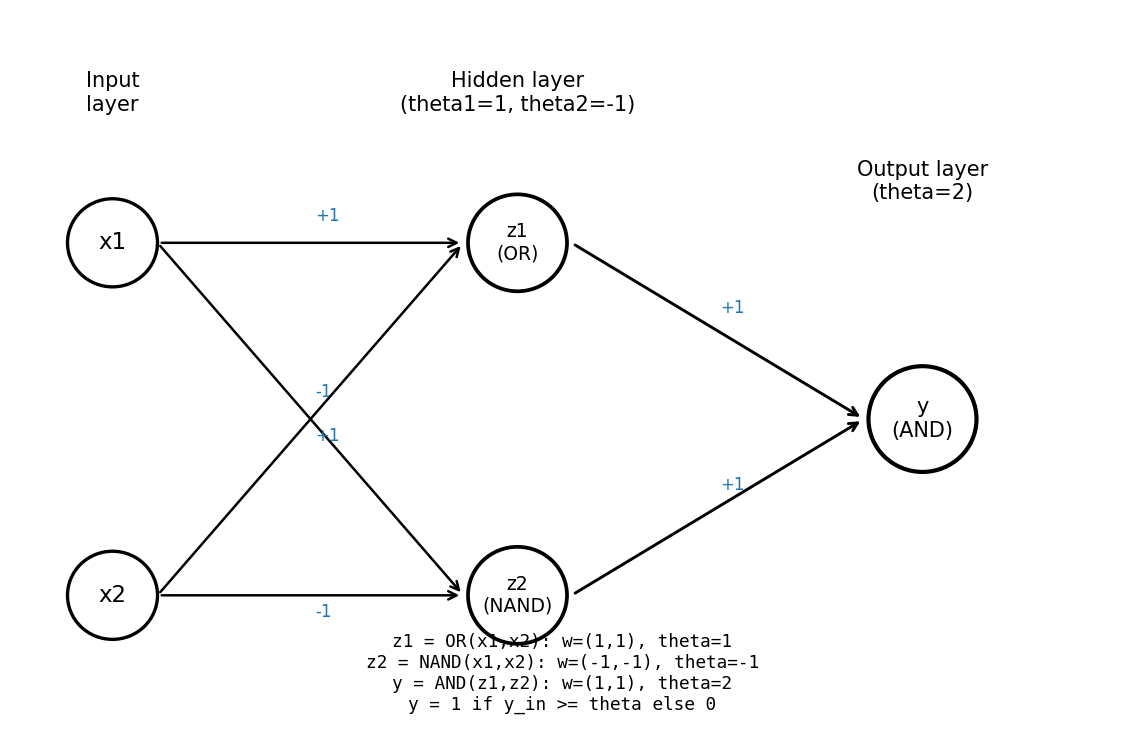
\includegraphics[width=0.85\textwidth]{outputs/mcp_xor_diagram.png}
\caption{McCulloch-Pitts network for XOR, built from OR and NAND hidden units combined by an AND output unit.}
\end{figure}

\begin{center}
\begin{tabular}{@{}rrrrrr@{}}
\toprule
$x_1$ & $x_2$ & $z_1$ (OR) & $z_2$ (NAND) & $y$ (AND) & Expected XOR \\
\midrule
0 & 0 & 0 & 1 & 0 & 0 \\
0 & 1 & 1 & 1 & 1 & 1 \\
1 & 0 & 1 & 1 & 1 & 1 \\
1 & 1 & 1 & 0 & 0 & 0 \\
\bottomrule
\end{tabular}
\end{center}

The network reproduces the XOR truth table exactly for all four input patterns.

\section*{7. Assignment 5 --- MLP for XOR using Backpropagation}

A 2-2-1 multilayer perceptron (two inputs, two hidden units, one output unit, all with sigmoid activation and a bias) was trained on the unipolar XOR truth table using the backpropagation formulas of Section 2, with $\alpha=0.5$. Random weight initialization matters for XOR: of 20 random seeds tried, 13 converged to the correct classification while 7 became stuck in a local minimum with mean-squared error around $0.13$ -- a well-known difficulty of training small MLPs on XOR with gradient descent. The best converged run (seed 1) was trained for 20000 epochs, reaching a final MSE of about $1.3\times10^{-4}$.

\begin{center}
\begin{tabular}{@{}rrrr@{}}
\toprule
$x_1$ & $x_2$ & Raw output & Predicted \\
\midrule
0 & 0 & 0.012 & 0 \\
0 & 1 & 0.987 & 1 \\
1 & 0 & 0.989 & 1 \\
1 & 1 & 0.010 & 0 \\
\bottomrule
\end{tabular}
\end{center}

\begin{figure}[H]
\centering
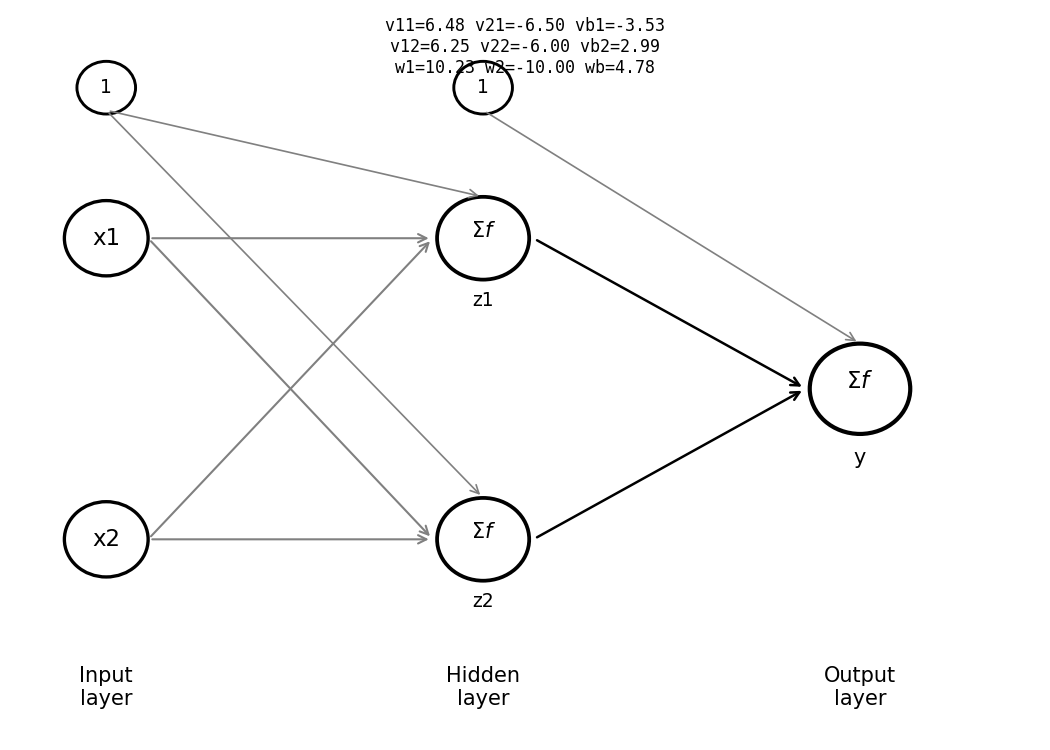
\includegraphics[width=0.92\textwidth]{outputs/xor_backprop_mlp_diagram.png}
\caption{MLP architecture used for XOR, annotated with the final learned weights and biases ($v$: input-to-hidden, $w$: hidden-to-output).}
\end{figure}

\begin{figure}[H]
\centering
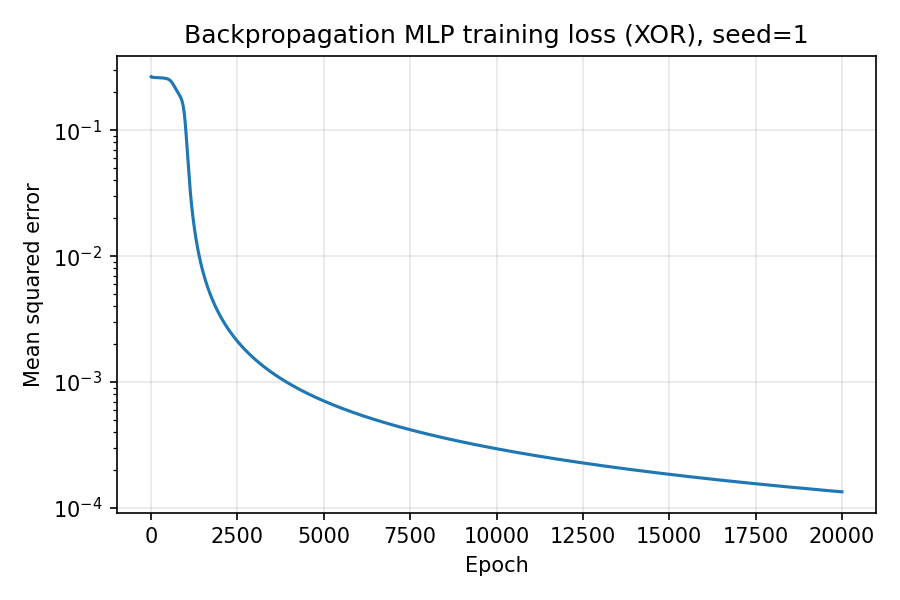
\includegraphics[width=0.46\textwidth]{outputs/xor_backprop_loss.png}
\hspace{0.02\textwidth}
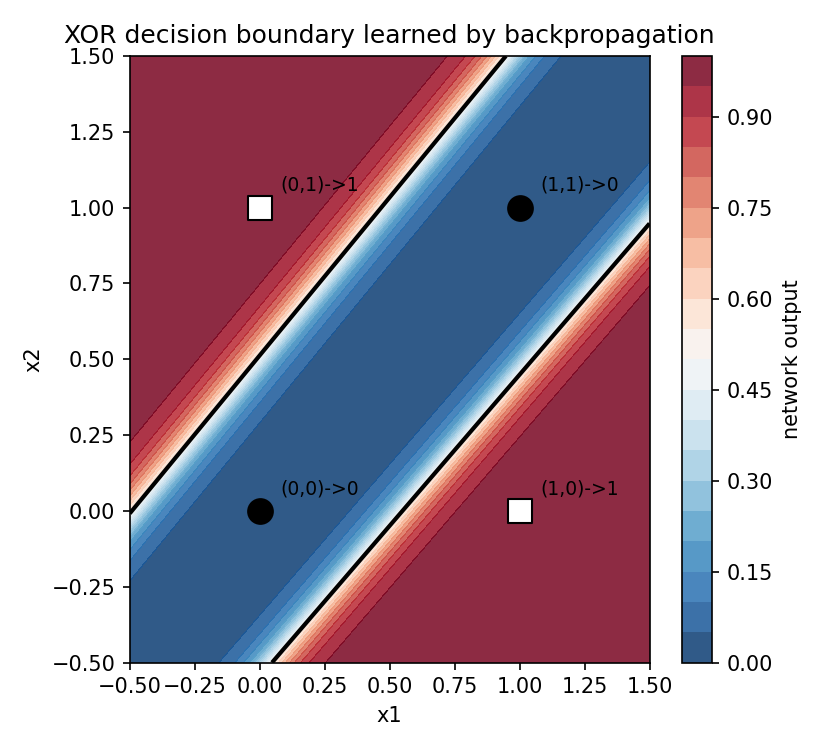
\includegraphics[width=0.46\textwidth]{outputs/xor_backprop_boundary.png}
\caption{Training loss (mean-squared error, log scale) and the learned decision boundary in input space. The boundary correctly separates the two same-class diagonal corners (0,0) and (1,1) from the two opposite-class corners (0,1) and (1,0), something no single straight line achieves for all four points simultaneously with one hidden layer of two units combining two half-planes.}
\end{figure}

The loss curve shows the characteristic behaviour of XOR training with sigmoid units: an initial slow plateau while the hidden units' decision boundaries are still poorly placed, followed by a rapid drop once the two hidden units align to carve out the diagonal band separating the two classes.

\section*{8. Conclusion}

A single Adaline unit trained with the delta rule successfully learns AND, OR, NAND and NOR under both the unipolar and bipolar encodings, since all four functions are linearly separable; the bipolar encoding converges substantially faster because it lets every input feature contribute to every weight update. The learning rate has a strong, non-monotonic effect on convergence speed: too small is slow, too large causes oscillation and failure to converge, and a moderate rate is best. XOR cannot be realized by a single such unit; it was solved in two different ways: a hand-designed McCulloch-Pitts network combining OR and NAND hidden units through an AND output unit, and a 2-2-1 MLP trained end-to-end with the backpropagation algorithm, which reached the same input-output mapping purely from data despite occasionally converging to a local minimum depending on the random initial weights.

The Python implementation, plots, JSON result summaries, and diagrams are included in the deliverables folder. The executable source is included in the \texttt{code} folder.

\newpage
\section*{Appendix: Source Code}

The core implementation is plain NumPy, no ML libraries were used, so the update rules are visible directly in the code. The plotting/diagram scripts (\texttt{make\_plots.py}, \texttt{draw\_diagrams.py}, \texttt{make\_backprop\_plots.py}) are not listed here since they are just matplotlib boilerplate for the figures above; they are included in the \texttt{code} folder.

\subsection*{A.1 adaline.py --- Assignments 1, 2, 3}
\lstinputlisting[style=code]{code/adaline.py}

\subsection*{A.2 param\_study.py --- Assignment 1 (parameter variation)}
\lstinputlisting[style=code]{code/param_study.py}

\subsection*{A.3 mcp\_xor.py --- Assignment 4}
\lstinputlisting[style=code]{code/mcp_xor.py}

\subsection*{A.4 backprop\_xor.py --- Assignment 5}
\lstinputlisting[style=code]{code/backprop_xor.py}

\end{document}
